%%%
%% v5.0 [2022/04/06]
\documentclass[fleqn]{ieej}
%\documentclass[letter,fleqn]{ieej}
%\documentclass[english,fleqn]{ieej}
%\documentclass[english,letter,fleqn]{ieej}
%\documentclass[comment,fleqn]{ieej}
%\documentclass[feature,fleqn]{ieej}
%\documentclass[foreword,fleqn]{ieej}
%\documentclass[essay,fleqn]{ieej}
%\usepackage{amsthm}
\usepackage{tabularx}
\usepackage[defaultsups]{newtxtext}
\usepackage[varg]{newtxmath}
\usepackage[superscript,nomove]{cite}
\usepackage[dvipdfmx]{graphicx}% for (u)platex
\usepackage[dvipdfmx]{hyperref}\usepackage{pxjahyper}% for (u)platex
\usepackage{comment}

\usepackage[top=30truemm,bottom=27truemm,left=18truemm,right=18truemm]{geometry} % 余白指定

\usepackage{multirow}

%\usepackage[subrefformat=parens]{subcaption}


\usepackage{float}
\makeatletter
\let\MYcaption\@makecaption
\makeatother

\usepackage{subcaption}
\captionsetup{compatibility=false}      

\makeatletter
\let\@makecaption\MYcaption
\makeatother

%\usepackage[T1]{fontenc}
%\usepackage{newpxtext, newpxmath}

\usepackage[T1]{fontenc}
\usepackage{lmodern}

%\usepackage[deluxe,expert]{otf} %ゴシック体に変更
%\renewcommand\kanjifamilydefault{\gtdefault} %gtdefault
%\renewcommand\familydefault{\sfdefault}

%\usepackage{graphicx}% for LuaLaTeX
%\usepackage[luatex,pdfencoding=auto]{hyperref}% for LuaLaTeX
\hypersetup{%
 setpagesize=false,
 colorlinks=true,
 %colorlinks=false,
 urlcolor=blue,
 citecolor=black,
 linkcolor=black,
}

\pagestyle{empty}%ページ番号なし

%\setcounter{page}{1}

\def\ClassFile{\texttt{ieej.cls}}
\def\PS{{\scshape Post\-Script}}
\def\AmSLaTeX{\leavevmode\hbox{$\cal A\kern-.2em\lower.376ex
 \hbox{$\cal M$}\kern-.2em\cal S$-\LaTeX}}
\def\BibTeX{{\rm B\kern-.05em{\sc i\kern-.025em b}\kern-.08em
 T\kern-.1667em\lower.7ex\hbox{E}\kern-.125emX}}

\FIELD{}
\YEAR{}
\NO{}
\jtitle[調整力市場参入時の自励変換装置制御]
       { 一次調整力の需給調整市場に参入する\\
       水電解装置が接続された自励変換装置の制御}
\etitle{Control by Self-commutated Converter Connected Electrolyzer Participating in Reserve Market of Primary Regulation}
\makeatletter
\if@english
\makeatother
 \authorlist{%
  %\authorentry[nakamura.yuta@nitech.ac.jp]{Yuta Nakamura}{}{NiTech}
  %\authorentry{Mutsumi Aoki}{}{NiTech}% [ABC]
 }
 %\affiliate[Nitech]
 % {	Nagoya Institute of Technology.\\
%	Gokiso-cho, Showa-ku, Nagoya, Aichi, 466-8555, Japan.}

\else
 \authorlist{%
  \authorentry[yuta.nakamura@mem.iee.or.jp]{中村 勇太*,}{Yuta Nakamura,}{N}{}
  \authorentry{青木 睦(名古屋工業大学)}{Mutsumi Aoki (Nagoya Institute of Technology)}{N}{}
 }
 %\affiliate[NiTech]
 % {名古屋工業大学\\ 〒466--8555\hskip1\zw 愛知県名古屋市昭和区御器所町}
 % {	Nagoya Institute of Technology.\\
%	Gokiso-cho, Showa-ku, Nagoya, Aichi, 466-8555, Japan.}
\fi
%\received{20XX}{XX}{XX}
%\revised{20XX}{XX}{XX}
\graphicspath{ {./National2024/} }

\begin{document}

%\begin{abstract}

%\end{abstract}
%\begin{jkeyword}
%  自励変換装置,可制御直流負荷,frequency-watt制御, 需給調整市場,水素
%\end{jkeyword}
%\begin{ekeyword}
%  self-commutated converter, controllable DC load, frequency-watt control, reserve market, hydrogen
%\end{ekeyword}


%\maketitle
\thispagestyle{empty}

\twocolumn[%
\begin{center}
{\fontsize{18pt}{28pt}\selectfont 需給調整市場に参入する複数の水電解装置システムの運用\\ーセル劣化のばらつきを考慮した最適運用ー} \\
\vspace{18pt}
{\fontsize{12pt}{18pt}\selectfont 中村 勇太*,青木 睦(名古屋工業大学)\\}
\vspace{18pt}
{\fontsize{9pt}{14pt}\selectfont Operation of System in Multiple Electrolyzers Participating in Reserve Market\\
                      - Optimal Operation Considering Degradation Variation in Cell Degradation -} \\
\vspace{1mm}
{\fontsize{9pt}{14pt}\selectfont Yuta Nakamura, Mutsumi Aoki (Nagoya Institute of Technology)\\ } 
\vspace{4mm}
\end{center}
]


\section{はじめに}\label{sec:intro}

\vspace{-2mm}

\fontsize{9pt}{14pt}\selectfont


自然変動電源の大量導入による電力系統の周波数変動対策として,
蓄電池をはじめとする需要家リソースを活用した需給調整力の提供が数多く検討されている。
%その対策として,系統に連系されている自励変換装置を用いた系統安定化制御が数多く検討されている。
著者らはこれまで,需要家リソースの中でも水電解装置に着目し,需給調整市場の枠組や要件に沿った,
水電解装置が連系されたシステムの運用法\cite{Nakamura_2021}や制御法\cite{Nakamura_2023}に関する検討を行った。

また近年では,水素生成コスト低減を目的としたシステムの大容量化に向け,
水電解装置そのものの大型化に加えて,水電解装置を並列化して系統連系させることが検討されつつある。
水電解装置の劣化は主に電解セルで生じるが,
その劣化を含めた負荷特性は,水電解装置の稼働状態やセル毎の個体差等,様々な要因によって異なる。
そのため,複数の水電解装置が並列化されている場合,システム全体として経済的に最適に運用するために,
水電解装置間で生じるセル劣化のばらつきを考慮する必要があるだろう。

そこで本稿では,需給調整市場に参入する複数の水電解装置システムにおいて,
水電解装置間のセル劣化のばらつきを考慮した最適運用法について検討する。

\vspace{-2mm}

\section{システムと想定する状況}\label{sec:system}

\vspace{-2mm}

<\ref{sec:system}・1>システム構成と運用方針  図\ref{fig:System}は本稿で想定するシステムの概要図を示している。
これは,既報\cite{Nakamura_2021} で検討したマイクログリッドのうちの水素生成設備部分に該当する。
具体的には,定格10MWの水電解装置2台および9MW一定負荷の補器類が電力系統に連系されている。

システムは受電点の有効電力を監視し,所望の水素需要を満たしつつ,
系統運用者からの需給調整の指令に従うように,水電解装置を個別に制御する。
詳細は既報\cite{Nakamura_2023}に譲る。

\begin{figure}[b]% fig.4  
      %\begin{minipage}{8cm}
      \begin{center}
      \setlength{\abovecaptionskip}{0mm} % 図キャプション上空行幅調整
      \setlength{\belowcaptionskip}{0mm} % 図キャプション下空行幅調整
      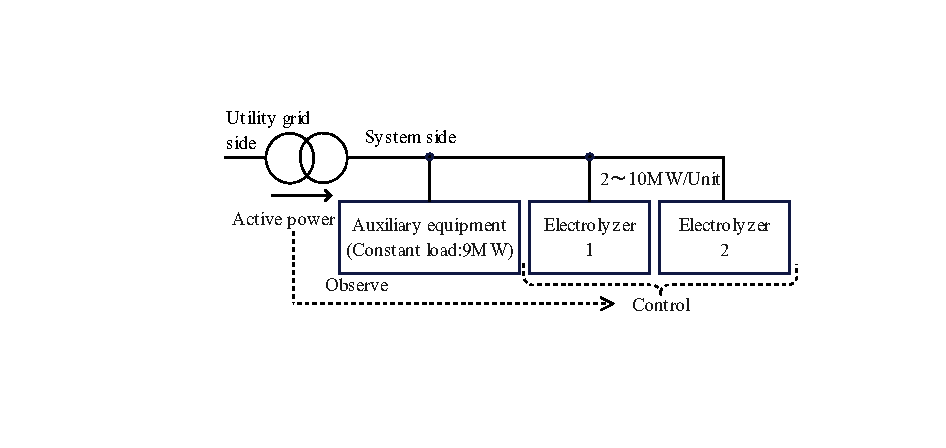
\includegraphics[width=8cm,height=3.5cm]{System_2units.pdf}  
      \textmc{図\ref{fig:System} 想定するシステムの概要図}  
      \caption{Summary of assumed system}\label{fig:System}
       
    \end{center}
    %\end{minipage}
    \begin{center}
      \setlength{\abovecaptionskip}{0mm} % 図キャプション上空行幅調整
      \setlength{\belowcaptionskip}{0mm} % 図キャプション下空行幅調整
      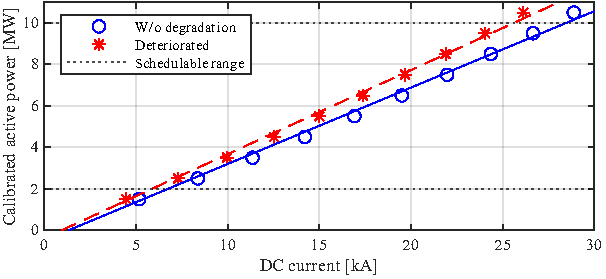
\includegraphics[width=8cm,height=3.8cm]{Current_power_curve.pdf}  
      \textmc{図\ref{fig:power_curve} 水電解装置の$I-P$特性}  
      \caption{$I-P$ characteristics of electrolyzer}\label{fig:power_curve}   
    \end{center}
\end{figure}

<\ref{sec:system}・2>水電解装置の劣化  
水電解装置の劣化は主に,電解セルの電流の大きさ,
電流が流れる時間・通電停止(装置停止)を含む電流変動の大きさ・サイクル数によって異なるとされる。
図\ref{fig:Polarization}は,本稿で想定するアルカリ型水電解装置の負荷特性を示している。
水電解装置の劣化により,同一のセル電流に対するセル電圧が実線から破線のように上昇する。

%劣化がない,本来の特性は図中の実線であるが,水電解装置の劣化が進むにつれて,破線のようにセル電圧が上昇する。



\vspace{-2mm}

\section{セル劣化を考慮した運用}\label{sec:proposed_method}

\vspace{-2mm}

<\ref{sec:proposed_method}・1>セル劣化を考慮した負荷特性の校正  
水電解装置単位で異なる劣化を考慮した運用を行うために,
水電解装置毎に負荷特性を校正する。
%水電解装置の負荷特性は通常,図\ref{fig:Polarization}のようにセル電流とセル電圧の関係($I-V$特性)で表されるが,
%システムとして運用計画策定できるよう,負荷の電流と水電解装置全体で消費する有効電力($I-P$特性)で表す。
図\ref{fig:power_curve}は,セル劣化を考慮した負荷の電流と水電解装置全体で消費する有効電力の特性($I-P$特性)を示している。
これは図\ref{fig:Polarization}の負荷をそれぞれ接続した,
単機の水電解装置のシステム\cite{Nakamura_2023}におけるシミュレーション(計測値)から算出したものであり,
各種電力損失も含まれている。

\begin{figure}[b]% fig.4  
  %\begin{minipage}{8cm}
  \begin{center}
  \setlength{\abovecaptionskip}{0mm} % 図キャプション上空行幅調整
  \setlength{\belowcaptionskip}{0mm} % 図キャプション下空行幅調整
  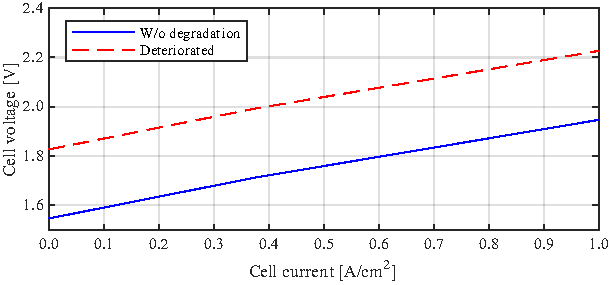
\includegraphics[width=8cm,height=3.8cm]{Polarization_curves.pdf}  
  \textmc{図\ref{fig:Polarization} 水電解装置の負荷特性}  
  \caption{Polarization curves of electrolyzer}\label{fig:Polarization}   
  \end{center}
%\end{minipage}
\end{figure}


<\ref{sec:proposed_method}・2>提案する運用法  
提案する運用法は,事前に求めた$I-P$特性に基づき,システムの運用コストが最小になる%運用計画を策定し,
計画に従って運用する手法である。
運用コストは,所望の水素需要を満たすために必要な買電コストから,
需給調整市場参入によって得られる収入を差し引いたコストであり,
運用計画はその運用コストを最小化する最適化問題を解くことで決定される。
制約条件は,下記の通りである。
\begin{itemize}
  \item 電力需給バランス制約        
  \item 水電解装置の出力上下限制約(2~10MW:図\ref{fig:power_curve} の点線)
  \item 水素需要・供給制約(1日で需要量を満たすように運用)
\end{itemize}

水電解装置の劣化を考慮しない場合の最適化問題は既報\cite{Nakamura_2021}を参照されたい。

\vspace{-2mm}

\section{数値試算による提案手法の有効性検証}\label{sec:simulation}

\vspace{-2mm}

%本稿では,提案手法による運用計画の有効性を示すために,
%数値シミュレーションを行った。
<\ref{sec:simulation}・1>試算条件  %運用コストを算出するための必要な
劣化の違いが計画に与える影響を明確できるように,
2つの水電解装置の負荷は,図\ref{fig:power_curve}に示す2つの$I-P$特性のうち,
劣化が無い(水電解装置1),劣化を有する(水電解装置2)特性をそれぞれ持たせた。
買電単価および調整力提供に対する単価($\Delta$ kW・kWh単価)は
既報\cite{Nakamura_2023}と同じ単価を用いた。
水素需要は,水電解装置の1日設備利用率が60\%程度になるように設定した。


<\ref{sec:simulation}・2>試算結果  
図\ref{fig:proposed}は提案手法,2つの水電解装置の運用結果を示している。
太線が各水電解装置の計画値(調整力算出のベースライン),
青色・赤線が出力下げ・上げ方向の調整力をそれぞれ示している。
多くの時間で,劣化が無い水電解装置1(図\ref{fig:proposed}(a))は定格出力をベースラインとし下げ方向の調整力,
劣化を有する水電解装置2(図\ref{fig:proposed}(b))は最低出力で出力上げ方向調整力を確保している。
一方,図\ref{fig:uniformity}は2つの$I-P$特性の平均を一律の特性として
計画させた手法(従来手法)の運用結果を示しているが,
各水電解装置が中間出力をベースラインとし,両方向の調整力を提供している。

表\ref{table:Economic}は,各手法の運用コストおよび水素コストの内訳を示している。
買電コストは劣化を考慮する提案手法が従来手法よりも低くなっている。
これは,劣化の優劣に応じて出力の配分を変えているため,
買電単価が高い17:30~19:00に一時的に出力を下げていることが原因である。
一方,従来手法では,劣化度合いに応じた出力配分がされていないため,全体として生成される水素量が少なく,
水素需要を満たすためにこの時間に出力を下げることができない。
その結果として,調整力提供に提供に対する収入は,購入電力量が多く調整代を確保しやすい従来手法が多いが,
運用コストおよびこのコストを水素生成量で除算した水素生成コストは提案手法が低い。%優れている。

さらに水電解装置の観点から見ても,
劣化のばらつきに応じて出力を配分し,劣化の進行を平準化する提案手法は合理的であると考えられる。

%通過電流が大きいほど劣化が進むことから,
%劣化が進行している水電解装置の出力を下げて,劣化が進行していない水電解装置のベース出力を上げるといった
%配分することは劣化を平準化する観点でも合理的であると考えられる。

%これより,水電解装置の劣化のばらつきを考慮して運用することで,
%より適切に運用できることが明らかになった。

\vspace{-2mm}

\section{おわりに}\label{sec:conclusion}

\vspace{-2mm}

本稿では,需給調整市場に参入する複数の水電解装置システムにおいて,
水電解装置間のセル劣化のばらつきを考慮した運用法について検討した。
今後は,水電解装置間のセル劣化のばらつきを考慮して系統運用者からの需給調整指令を配分するといった,
システム全体の制御法を検討する予定である。

%水電解装置以外の需要家リソースを有するシステムでの各リソースの劣化を考慮した運用法や,
%系統運用者からの需給調整指令を水電解装置間のセル劣化のばらつきを考慮して配分するといった,
%適切にシステム全体を制御する方法について検討する予定である。

\begin{figure}[t]% fig.4  
  \begin{center}
    \begin{minipage}{8cm}
      \begin{center}
      \setlength{\abovecaptionskip}{0mm} % 図キャプション上空行幅調整
      \setlength{\belowcaptionskip}{0mm} % 図キャプション下空行幅調整
      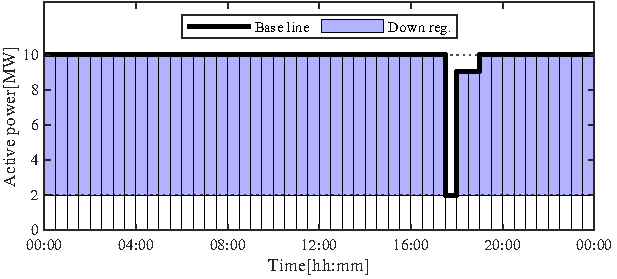
\includegraphics[width=8cm,height=3.8cm]{proposed_method_E1.pdf}  
      \subcaption{W/o degradation Electrolyser(Electrolyser 1)}
    \end{center}
    \end{minipage}
 
    \begin{minipage}{8cm}
      \begin{center}
      \setlength{\abovecaptionskip}{0mm} % 図キャプション上空行幅調整
      \setlength{\belowcaptionskip}{0mm} % 図キャプション下空行幅調整
      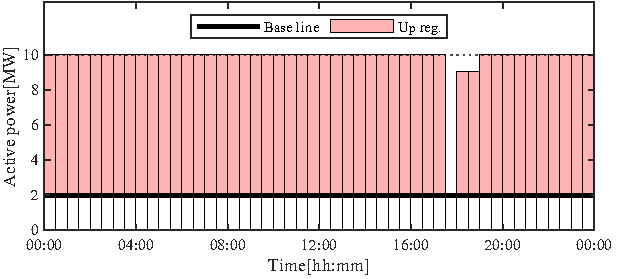
\includegraphics[width=8cm,height=3.8cm]{proposed_method_E2.pdf}  
      \subcaption{Degradation Electrolyser(Electrolyser 2)}
    \end{center}
    \end{minipage}

  
  \textmc{図\ref{fig:proposed} 提案手法における水電解装置の運用}  
  \caption{Operation of electrolysers in proposed method}\label{fig:proposed}
  

  \begin{minipage}{8cm}
    \begin{center}
    \setlength{\abovecaptionskip}{0mm} % 図キャプション上空行幅調整
    \setlength{\belowcaptionskip}{0mm} % 図キャプション下空行幅調整
    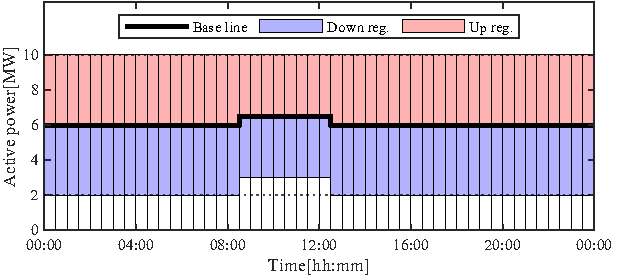
\includegraphics[width=8cm,height=3.8cm]{uniformity_shedule.pdf}  
    %\subcaption{Uniformity operation}
  \end{center}
  \end{minipage}


  \textmc{図\ref{fig:uniformity} 劣化を考慮しない一律の水電解装置の運用}  
  \caption{Uniformity operation of electrolysers}\label{fig:uniformity}
  \end{center}
\end{figure}

\begin{table}[t]
  \begin{center}
  \textmc{表\ref{table:Economic} 運用コストおよび水素単価}
  \caption{Operation cost and hydrogen price}
  \label{table:Economic}
    %\begin{minipage}{8cm}
      \begin{center}
        \setlength{\abovecaptionskip}{0mm} % 図キャプション上空行幅調整
        \setlength{\belowcaptionskip}{0mm} % 図キャプション下空行幅調整
        %\subcaption{Differece active power between refrerence and mesurement}
        \begin{tabular}{|c||r|r|}
          \hline
          Items &
          \begin{tabular}{c} Considering\\degradation \end{tabular}&
          \begin{tabular}{c} Uniformity\\operation \end{tabular} \\

          \hline \hline          
          Energy purchase[$10^4$JPY]  & 476.4 & 485.4 \\
          \hline
          Income procurement regulation [$10^4$JPY]  & 24.9 & 25.0\\
          \hline
          Operation cost[$10^4$JPY] (A)  & 451.5 &460.4\\
          \hline       
          Hydrogen supply amount [Nm$^3$] (B) &  \multicolumn{2}{c|}{57,600} \\
          \hline
          Hydrogen price [JPY/Nm$^3$](=A/B) & 78.4  & 79.9\\

          \hline
        \end{tabular}
      \end{center}
    %\end{minipage}
  \end{center}  
\end{table}

%\vspace{-2mm}

\acknowledgment データの提供や助言を頂いた,旭化成株式会社 加戸 良英 氏,富士電機株式会社 壹岐 浩幸 氏に厚く感謝の意を表する。

\vspace{-2mm}

\bibliographystyle{junsrt} %参考文献を引用順に
\begin{thebibliography}{99}
 
  \bibitem{Nakamura_2021}
  中村他, 電学論B, 141 巻, 2 号, pp. 56-66 (2021)

  \bibitem{Nakamura_2023} 
  中村他, 電気学会B部門大会,16 (2023)
\end{thebibliography}


\end{document}